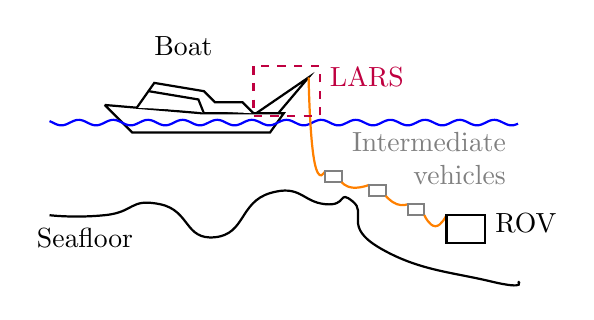
\begin{tikzpicture}[scale=0.7]
    % Boat
    \filldraw[fill=white, draw=black, thick] (0,0) -- (.5,-.5) -- (3.,-.5) -- (3.25,-0.15) -- (1.75,-0.15) -- (0,0);
    \filldraw[fill=white, draw=black, thick] (0.583,-0.05) -- (0.9,0.4) -- (1.8,0.25) -- (2.,0.05) -- (2.5,0.05) -- (2.7,-0.15);
    \filldraw[fill=white, draw=black, thick] (0.8,0.25) -- (1.7,0.1) -- (1.8,-0.15) ;
    \draw[thick, black] (2.75,-0.15) -- (3.7,0.5) -- (3.15,-0.15) ;
    \node[above, xshift=1.cm, yshift=0.5cm] {Boat};
    % Surface
    \draw[thick, blue] plot[domain=-1:7.5, samples=300]  (\x,{0.05*sin(\x*10 r)-0.32});
    % Cable
    \draw[thick, orange] plot[smooth, tension=1] coordinates{(3.7,0.5) (3.8,-1.) (4.,-1.2)};
    \filldraw[fill=white, draw=gray, thick] (4.,-1.2) rectangle (4.3, -1.4) node[right, xshift=0.cm, yshift=0.3cm, align=right, gray] {Intermediate\\vehicles};
    \draw[thick, orange] plot[smooth, tension=1] coordinates{(4.3, -1.4) (4.5,-1.5) (4.8,-1.45)};
    \filldraw[fill=white, draw=gray, thick] (4.8,-1.45) rectangle (5.1, -1.65);
    \draw[thick, orange] plot[smooth, tension=1] coordinates{(5.1, -1.65) (5.3,-1.8) (5.5,-1.8)};
    \filldraw[fill=white, draw=gray, thick] (5.5,-1.8) rectangle (5.8, -2.);
    \draw[thick, orange] plot[smooth, tension=1] coordinates{(5.8, -2.) (6.0,-2.2) (6.2, -2)};
    \filldraw[fill=white, draw=black, thick] (6.2, -2) rectangle (6.9, -2.5) node[right, yshift=0.25cm] {ROV};
    % LARS
    \draw[thick, purple, dashed] (2.7, 0.7) rectangle (3.9, -0.2) node[right, yshift=0.5cm] {LARS};
    % seabed
    \draw[thick, black] plot[smooth, tension=1] coordinates{(-1, -2.) (0,-2) (1, -1.8) (2, -2.4) (3, -1.6) (4., -1.8) (4.5, -1.75) (5, -2.6) (7, -3.2) (7.5, -3.2)} node[below, xshift=-5.5cm, yshift=0.8cm] {Seafloor};
\end{tikzpicture}